\section{Appendix : study of sign of roots in the case of linearization with $u_0 \neq 0$ (only for the dispersive equation)}

\indent The roots of \eqref{eq:pol3} are

\begingroup
\scriptsize
\begin{equation}
	\label{eq:lambdaExacts}
	\begin{aligned}
	&& \lambda_1\left( {{h_0}}, {{u_0}}, s \right) = & \frac{2^{\frac{1}{3}} \left(-\frac{{{h_0}}^{2} {{u_0}}^{3}}{2 \, {{h_0}}^{2} s^{3} - 81 \, s {{u_0}}^{2} - 9 \, \sqrt{-4 \, {{h_0}}^{2} s^{2} + 81 \, {{u_0}}^{2}} s {{u_0}}}\right)^{\frac{1}{3}} s^{2}}{3 \, {{u_0}}^{2}} + \\
	&& & {\left(\frac{\sqrt{-4 \, {{h_0}}^{2} s^{2} + 81 \, {{u_0}}^{2}} s}{6 \, {{h_0}}^{2} {{u_0}}^{2}} - \frac{2 \, {{h_0}}^{2} s^{3} - 81 \, s {{u_0}}^{2}}{54 \, {{h_0}}^{2} {{u_0}}^{3}}\right)}^{\frac{1}{3}} - \frac{s}{3 \, {{u_0}}} \\
	&& \lambda_2\left( {{h_0}}, {{u_0}}, s \right) = & -\frac{1}{12} \cdot 2^{\frac{2}{3}} {\left(i \, \sqrt{3} + 1\right)} \left(-\frac{2 \, {{h_0}}^{2} s^{3} - 81 \, s {{u_0}}^{2} - 9 \, \sqrt{-4 \, {{h_0}}^{2} s^{2} + 81 \, {{u_0}}^{2}} s {{u_0}}}{{{h_0}}^{2} {{u_0}}^{3}}\right)^{\frac{1}{3}}\\
	&& & + \frac{2^{\frac{1}{3}} \left(-\frac{{{h_0}}^{2} {{u_0}}^{3}}{2 \, {{h_0}}^{2} s^{3} - 81 \, s {{u_0}}^{2} - 9 \, \sqrt{-4 \, {{h_0}}^{2} s^{2} + 81 \, {{u_0}}^{2}} s {{u_0}}}\right)^{\frac{1}{3}} s^{2} {\left(i \, \sqrt{3} - 1\right)}}{6 \, {{u_0}}^{2}} - \frac{s}{3 \, {{u_0}}} \\
	&& \lambda_3\left( {{h_0}}, {{u_0}}, s \right) = & \frac{1}{12} \cdot 2^{\frac{2}{3}} {\left(i \, \sqrt{3} - 1\right)} \left(-\frac{2 \, {{h_0}}^{2} s^{3} - 81 \, s {{u_0}}^{2} - 9 \, \sqrt{-4 \, {{h_0}}^{2} s^{2} + 81 \, {{u_0}}^{2}} s {{u_0}}}{{{h_0}}^{2} {{u_0}}^{3}}\right)^{\frac{1}{3}} +\\
	&& & \frac{2^{\frac{1}{3}} \left(-\frac{{{h_0}}^{2} {{u_0}}^{3}}{2 \, {{h_0}}^{2} s^{3} - 81 \, s {{u_0}}^{2} - 9 \, \sqrt{-4 \, {{h_0}}^{2} s^{2} + 81 \, {{u_0}}^{2}} s {{u_0}}}\right)^{\frac{1}{3}} s^{2} {\left(-i \, \sqrt{3} - 1\right)}}{6 \, {{u_0}}^{2}} - \frac{s}{3 \, {{u_0}}}
	\end{aligned}
\end{equation}
\endgroup

\indent A Taylor expansion of these roots around $s = 0$ give

\begin{equation}
	\label{eq:taylor3}
	\begin{aligned}
		&& \lambda_1\left( {{h_0}}, {{u_0}}, s \right) = & \frac{3^{\frac{1}{3}} s^{\frac{1}{3}}}{{{h_0}}^{\frac{2}{3}} {{u_0}}^{\frac{1}{3}}} + \mathcal{O}(s) \\
		&& \lambda_2\left( {{h_0}}, {{u_0}}, s \right) = & \frac{2^{\frac{2}{3}} {\left(-i \cdot 6^{\frac{1}{3}} \sqrt{3} {{h_0}}^{\frac{1}{3}} {{u_0}}^{\frac{2}{3}} - 6^{\frac{1}{3}} {{h_0}}^{\frac{1}{3}} {{u_0}}^{\frac{2}{3}}\right)} s^{\frac{1}{3}}}{4 \, {{h_0}} {{u_0}}} + \mathcal{O}(s) = \\
		&& = & -C sign(u) s^{\frac{1}{3}} \left( \frac{1}{2} + i\frac{\sqrt{3}}{2}\right) + \mathcal{O}(s) = \\
		&& = & -C sign(u) s^{\frac{1}{3}} e^{i\frac{\pi}{3}} + \mathcal{O}(s) \\
		&& \lambda_3\left( {{h_0}}, {{u_0}}, s \right) = & \frac{2^{\frac{2}{3}} {\left(i \cdot 6^{\frac{1}{3}} \sqrt{3} {{h_0}}^{\frac{1}{3}} {{u_0}}^{\frac{2}{3}} - 6^{\frac{1}{3}} {{h_0}}^{\frac{1}{3}} {{u_0}}^{\frac{2}{3}}\right)} s^{\frac{1}{3}}}{4 \, {{h_0}} {{u_0}}} + \mathcal{O}(s) = \\
		&& = & C sign(u) s^{\frac{1}{3}} \left( -\frac{1}{2} + i\frac{\sqrt{3}}{2}\right) + \mathcal{O}(s) = \\
		&& = & C sign(u) s^{\frac{1}{3}} e^{i\frac{2\pi}{3}} + \mathcal{O}(s) \\
	\end{aligned}
\end{equation}

\noindent where

\begin{equation*}
	C = \frac{\left(24h_0u_0^2\right)^{\frac{1}{3}}}{2h_0|u_0|} > 0
\end{equation*}

\indent The Laplace frequencies $s$ are supposed to have positive real part. Writing $s = \rho e ^{i\theta}$, that implies

\begin{equation*}
	\theta \in \left] -\frac{\pi}{2}, \frac{\pi}{2} \right[
\end{equation*}

\indent and therefore

\begin{equation}
\label{eq:domaineAngles}
\begin{gathered}
	\frac{\theta}{3} \in \left] -\frac{\pi}{6}, \frac{\pi}{6} \right[ \\
	\frac{\theta}{3} + \frac{\pi}{3} \in \left] \frac{\pi}{6}, \frac{\pi}{2} \right[ \\
	\frac{\theta}{3} + \frac{2\pi}{3} \in \left] \frac{\pi}{2}, \frac{5\pi}{6} \right[
\end{gathered}
\end{equation}

\indent Truncating the Taylor expansions \eqref{eq:taylor3} at the first term and using the trigonometric form of $s$, we have

\begin{equation}
	\label{eq:seriesTrunc}
	\begin{aligned}
	\lambda_1\left( {{h_0}}, {{u_0}}, s \right) = & \frac{3^{\frac{1}{3}} \rho^{\frac{1}{3}}}{{{h_0}}^{\frac{2}{3}} {{u_0}}^{\frac{1}{3}}} e^{i\frac{\theta}{3}} \\
	\lambda_2\left( {{h_0}}, {{u_0}}, s \right) = & -C sign(u) \rho^{\frac{1}{3}} e^{i \left( \frac{\theta}{3}  + \frac{\pi}{3} \right)} \\
	\lambda_3\left( {{h_0}}, {{u_0}}, s \right) = & C sign(u) \rho^{\frac{1}{3}} e^{i \left( \frac{\theta}{3}  + \frac{2\pi}{3} \right)}
	\end{aligned}
\end{equation}

\indent From \eqref{eq:domaineAngles} and \eqref{eq:seriesTrunc}, it is clear that

\begin{equation*}
	sign(Re(\lambda_1)) = sign(u),  \qquad sign(Re(\lambda_2)) = -sign(u), \qquad sign(Re(\lambda_3)) = -sign(u)
\end{equation*}

\indent As an example, the figures \ref{fig:cas1} to \ref{fig:cas3} show the real part of the roots (computed using the exact expressions \eqref{eq:lambdaExacts}) in function of $h_0$ for some fixed values of $s$ and $u_0$ (the values were chosen varying the magnitude and the sign of $Im(s)$ and $u_0$).

\begingroup
	\noindent
	\begin{minipage}{.5\linewidth}
		\centering
		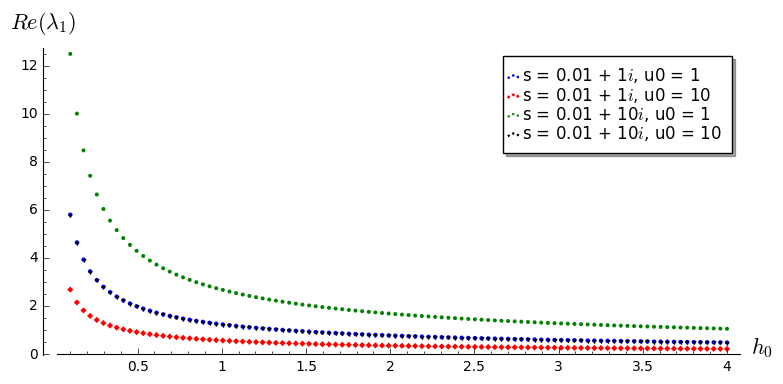
\includegraphics[scale=.35]{{Figures/LinDispersive/l1A}.png}
		\captionof{subfigure}{$Re(\lambda_1)$}
	\end{minipage}
	\begin{minipage}{.5\linewidth}
		\centering
		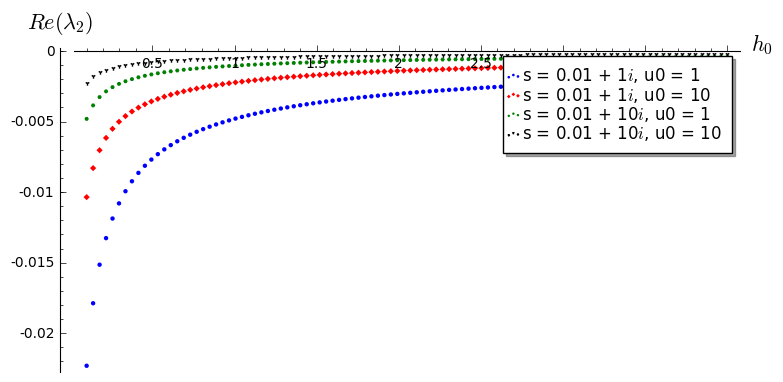
\includegraphics[scale=.35]{{Figures/LinDispersive/l2A}.png}
		\captionof{subfigure}{$Re(\lambda_2)$}
	\end{minipage}
	\begin{minipage}{1.\linewidth}
		\centering
		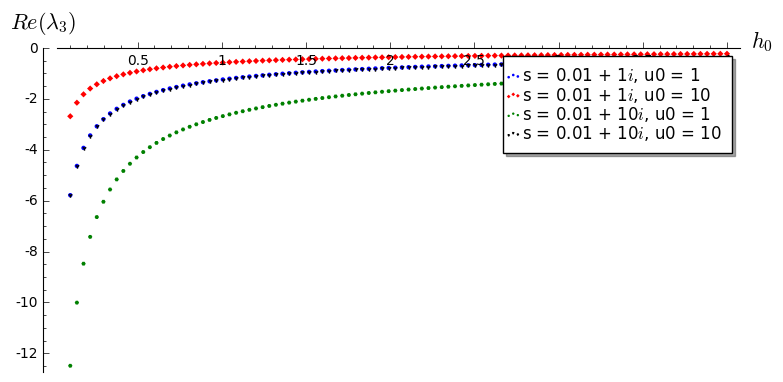
\includegraphics[scale=.35]{{Figures/LinDispersive/l3A}.png}
		\captionof{subfigure}{$Re(\lambda_3)$}
	\end{minipage}
	\captionof{figure}{Cas 1 \label{fig:cas1}}
\endgroup

\begingroup
	\noindent
	\begin{minipage}{.5\linewidth}
		\centering
		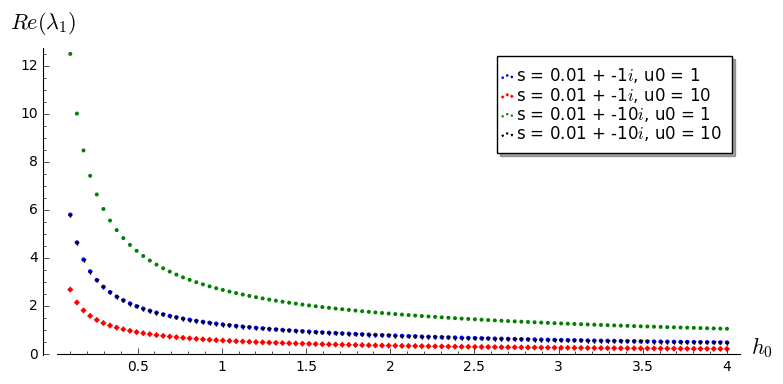
\includegraphics[scale=.35]{{Figures/LinDispersive/l1B}.png}
		\captionof{subfigure}{$Re(\lambda_1)$}
	\end{minipage}
	\begin{minipage}{.5\linewidth}
		\centering
		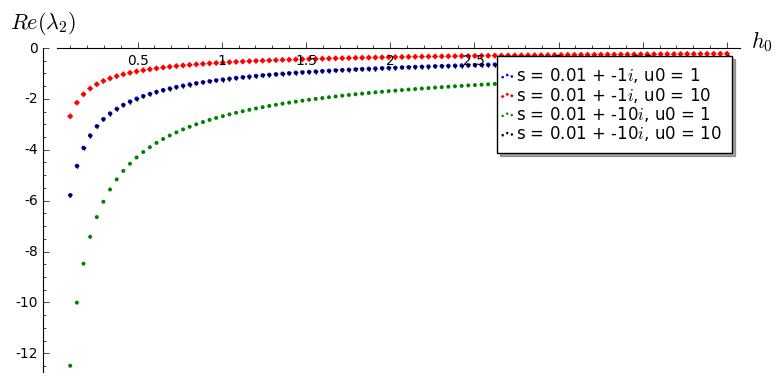
\includegraphics[scale=.35]{{Figures/LinDispersive/l2B}.png}
		\captionof{subfigure}{$Re(\lambda_2)$}
	\end{minipage}
	\begin{minipage}{\linewidth}
		\centering
		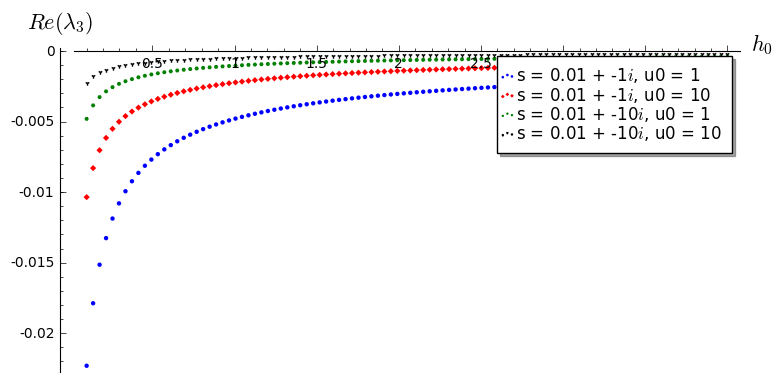
\includegraphics[scale=.35]{{Figures/LinDispersive/l3B}.png}
		\captionof{subfigure}{$Re(\lambda_3)$}
	\end{minipage}
	\captionof{figure}{Cas 2 \label{fig:cas2}}
\endgroup

\begingroup
\noindent
	\begin{minipage}{.5\linewidth}
		\centering
		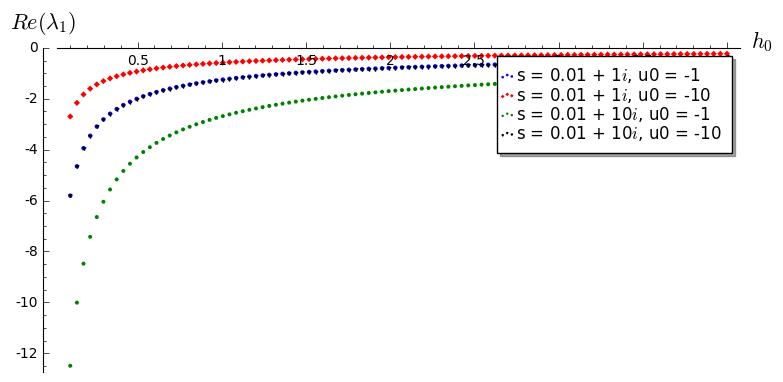
\includegraphics[scale=.35]{{Figures/LinDispersive/l1C}.png}
		\captionof{subfigure}{$Re(\lambda_1)$}
	\end{minipage}
	\begin{minipage}{.5\linewidth}
		\centering
		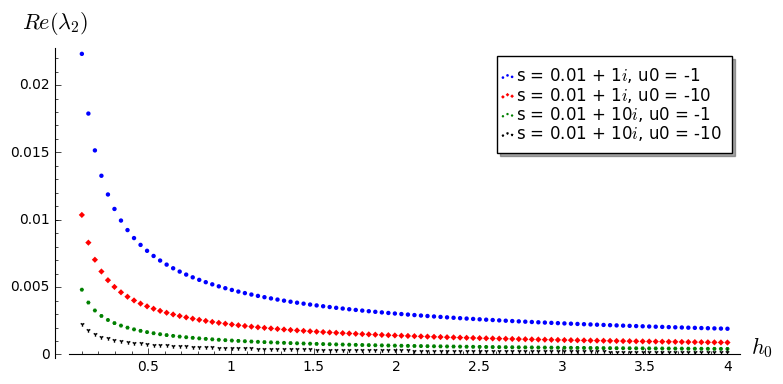
\includegraphics[scale=.35]{{Figures/LinDispersive/l2C}.png}
		\captionof{subfigure}{$Re(\lambda_2)$}
	\end{minipage}
	\begin{minipage}{\linewidth}
		\centering
		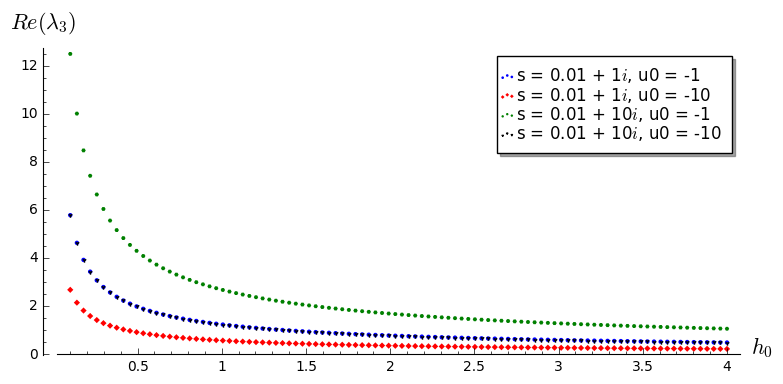
\includegraphics[scale=.35]{{Figures/LinDispersive/l3C}.png}
		\captionof{subfigure}{$Re(\lambda_3)$}
	\end{minipage}
	\captionof{figure}{Cas 3 \label{fig:cas3}}
\endgroup